%=====================================================================================
\section{Validity: do score changes track market surprises?}\label{sec:validity}

\subsection{Specification}

If a stance score measures what the statement says about future policy, changes in the score should move
with the market's reading of the announcement. I estimate
\begin{equation}
y_t = \alpha + \beta\,\text{dScore}_t + \varepsilon_t
\end{equation}
over statements up to December 2023, where $y_t$ is a market outcome at statement $t$. Standard errors
are Newey--West \citep{newey1987} with a Bartlett kernel and $\lfloor 4(n/100)^{2/9}\rfloor$ lags, a common
rule of thumb associated with \citet{newey1994}, which is \R{prim.lag} meetings in these samples;
$p$-values use the Student $t$ distribution.

The \emph{primary specification} uses MPS as the outcome, Fable's dScore, the policy corpus and hold
meetings only, with no controls. Hold meetings are the natural test: at a rate change both the score and
the surprise move with the decision, so their correlation could simply reflect the decision, which no
LLM is needed to read. MPS is measured in a 30-minute window and so isolates the announcement.

This specification was frozen on 3 October 2026, after earlier versions had been estimated and seen. The
choice of hold meetings, of MPS as the outcome, of the five-prompt consensus over a single prompt, of
whether to control for the rate change, and of the corpus definition were all made after looking at
results. The corpus definition, in particular, followed an independent review of the code which found
that seven non-policy notices, then coded as hold meetings, drove the earlier daily-yield results. The
adjusted $p$-values below correct for the twelve regressions in Fable's primary family. They do not
correct for this search, so even they overstate the evidence. The main analysis run reports
\R{regs.csv} regression coefficients with their tests (Appendix~\ref{app:disclose}), and the checks in
this section add more.

\subsection{The primary result}

\begin{table}[t]
\centering
\caption{The primary specification and its family}\label{tab:primary}
\small
% generated by paper/make_tables.py - do not edit
\begin{tabular}{@{}lll rrrr rr@{}}
\toprule
Outcome & Meetings & Control & $n$ & $\hat\beta$ & NW $t$ & $p$ & Holm $p$ & Bonferroni $p$ \\
\midrule
MPS & all & -- & 198 & 0.049 & 3.02 & 0.003 & 0.034 & 0.034 \\
\textbf{MPS} & \textbf{hold} & \textbf{--} & \textbf{132} & \textbf{0.033} & \textbf{2.39} & \textbf{0.018} & \textbf{0.199} & \textbf{0.217} \\
MPS & all & change\_bp & 198 & 0.036 & 2.27 & 0.025 & 0.245 & 0.294 \\
$d_{10}$ (bp) & hold & -- & 120 & 5.20 & 1.74 & 0.084 & 0.756 & 1.000 \\
$d_{10}$ (bp) & all & change\_bp & 173 & 4.39 & 1.52 & 0.130 & 1.000 & 1.000 \\
$d_{10}$ (bp) & all & -- & 173 & 4.27 & 1.44 & 0.151 & 1.000 & 1.000 \\
$d_2$ (bp) & all & change\_bp & 173 & 4.93 & 1.41 & 0.160 & 1.000 & 1.000 \\
$d_2$ (bp) & all & -- & 173 & 5.02 & 1.41 & 0.162 & 1.000 & 1.000 \\
$d_2$ (bp) & hold & -- & 120 & 3.77 & 1.03 & 0.306 & 1.000 & 1.000 \\
MPS\_ORTH & all & -- & 189 & 0.014 & 0.79 & 0.431 & 1.000 & 1.000 \\
MPS\_ORTH & hold & -- & 125 & 0.011 & 0.69 & 0.490 & 1.000 & 1.000 \\
MPS\_ORTH & all & change\_bp & 189 & 0.010 & 0.56 & 0.578 & 1.000 & 1.000 \\
\midrule
MPS, 2003+ sample & hold & -- & 120 & 0.038 & 2.65 & 0.009 & -- & -- \\
\bottomrule
\end{tabular}

\tabnote{\emph{Notes:} Fable consensus dScore, policy corpus, statements to December 2023. Each row is one
regression of the outcome on dScore (and the rate change in basis points, where shown). The family is
the twelve combinations of four outcomes (MPS, MPS\_ORTH, $d_2$, $d_{10}$) and three samples; Holm and
Bonferroni adjust for these twelve tests only. Newey--West $t$ with \R{prim.lag} lags. The primary
specification is in bold. The last row repeats it on the 2003+ meetings that also have daily yields.}
\end{table}

Table~\ref{tab:primary} reports the primary regression and its family. On \R{prim.n} hold meetings from
\R{prim.first} to \R{prim.last}, the slope is \R{prim.beta} percentage points of MPS per unit of dScore,
with a Newey--West $t$ of \R{prim.t} ($p=\R{prim.p}$) and an $R^2$ of \R{prim.r2}. The OLS and
heteroskedasticity-robust $t$-statistics are similar (\R{prim.tols} and \R{prim.thc}). In economic terms
the relation is small: a one-standard-deviation change in dScore (\R{fable.sd}) goes with
\R{prim.persd} percentage points of MPS, about \R{prim.persd.ratio} of the standard deviation of MPS at
hold meetings. On the \R{prim03.n} hold meetings from 2003 onwards, which also have daily yields, the
$t$-statistic is \R{prim03.t}.

The result does not survive a correction for multiple testing. Its Holm-adjusted $p$-value
\citep{holm1979} over the twelve tests is \R{fam.MPS.hold.none.holm} (Bonferroni
\R{fam.MPS.hold.none.bonf}). The only regression in the family that survives is MPS on all meetings
($t=\R{fam.MPS.all.none.t}$, Holm $p=\R{fam.MPS.all.none.holm}$). That regression includes the rate
decisions; controlling for the size of the rate change lowers its $t$ to \R{fam.MPS.all.ctrl.t}.

\subsection{Other outcomes and other scores}

\begin{table}[t]
\centering
\caption{Hold meetings: slopes on dScore by outcome and score}\label{tab:secondary}
\footnotesize
\setlength{\tabcolsep}{4.5pt}
% generated by paper/make_tables.py - do not edit
\begin{tabular}{@{}l r ccccccc@{}}
\toprule
Outcome & $n$ & Fable & Gemini & Dictionary & Fable P1 & P1 blinded & P1 paraphr. & GPT-4 P1 \\
\midrule
MPS & 132 & 0.033 & 0.003 & $-$0.010 & 0.026 & 0.017 & 0.014 & $-$0.006 \\
 & & (2.39) & (0.27) & ($-$0.99) & (2.20) & (1.43) & (0.90) & ($-$0.63) \\
\addlinespace[3pt]
MPS\_ORTH & 125 & 0.011 & $-$0.009 & $-$0.021 & 0.008 & $-$0.001 & $-$0.009 & $-$0.016 \\
 & & (0.69) & ($-$0.91) & ($-$1.75) & (0.55) & ($-$0.06) & ($-$0.53) & ($-$1.92) \\
\addlinespace[3pt]
$t_2$ (30-min, bp) & 132 & 3.76 & 0.03 & $-$1.52 & 2.66 & 1.72 & 1.42 & $-$1.11 \\
 & & (2.05) & (0.03) & ($-$1.39) & (1.74) & (1.12) & (0.74) & ($-$1.03) \\
\addlinespace[3pt]
$t_{10}$ (30-min, bp) & 132 & 2.98 & 0.06 & $-$0.54 & 1.85 & 1.45 & 0.96 & $-$0.61 \\
 & & (2.10) & (0.10) & ($-$0.66) & (1.75) & (1.38) & (0.68) & ($-$0.94) \\
\addlinespace[3pt]
$d_2$ (daily, bp) & 120 & 3.77 & $-$2.26 & $-$0.36 & 2.21 & 0.06 & $-$0.97 & $-$2.55 \\
 & & (1.03) & ($-$1.29) & ($-$0.17) & (0.74) & (0.02) & ($-$0.26) & ($-$1.88) \\
\addlinespace[3pt]
$d_{10}$ (daily, bp) & 120 & 5.20 & $-$0.15 & 1.70 & 3.18 & 1.44 & 1.10 & $-$0.05 \\
 & & (1.74) & ($-$0.11) & (0.87) & (1.40) & (0.61) & (0.37) & ($-$0.04) \\
\bottomrule
\end{tabular}

\tabnote{\emph{Notes:} Slope of each outcome on dScore with Newey--West $t$ in parentheses; hold meetings,
policy corpus, statements to December 2023. Fable and Gemini: five-prompt consensus with prompt fixed
effects. Dictionary: word-count score. Fable P1: re-score with prompt P1 on the cleaned original text; P1
blinded and P1 paraphrased: the same prompt on the blinded and paraphrased versions. GPT-4: prompt P1;
it lacks a few statements, so its $n$ is up to three lower. MPS in percentage points per unit of dScore,
yields in basis points.}
\end{table}

Table~\ref{tab:secondary} reports every outcome for every score on hold meetings. Three facts stand out.

First, Fable's dScore is unrelated to MPS\_ORTH ($t=\R{hold.fable.MPS_ORTH.t}$), the part of the surprise
that \citet{bauer2023reassessment} show is not predictable from macroeconomic and financial data released
before the meeting. Its relation is with the predictable part: on the same \R{extra.predpart.n} meetings,
regressing MPS minus MPS\_ORTH on dScore gives $t=\R{extra.predpart.t}$ (Table~\ref{tab:extra}; an
exploratory check). A model that knows the economic context of each meeting would pick up exactly that
component, whether it reads it from the text or recalls it.

Second, the 30-minute yield changes give $t$-statistics of \R{hold.fable.t2.t} ($t_2$) and
\R{hold.fable.t10.t} ($t_{10}$), close to the MPS result. They are not independent evidence: on hold
meetings their correlation with MPS is \R{desc.corr.MPS.t2} and \R{desc.corr.MPS.t10}. The daily yield
changes are not significantly related to dScore ($t$ of \R{hold.fable.d2.t} for $d_2$ and
\R{hold.fable.d10.t} for $d_{10}$). Daily changes also contain the day's other news, so they are a noisier
outcome.

Third, no other score shows a relation. Gemini's dScore has $t$-statistics between
\R{hold.gemini.d2.t} and \R{hold.gemini.MPS.t} on the six outcomes, the dictionary's are of either sign
and none is significant, and GPT-4's are all negative or near zero. Fable's own single-prompt re-score on
the cleaned text gives an MPS $t$ of \R{hold.clean.MPS.t}; on blinded and paraphrased text the same
prompt gives \R{hold.blind.MPS.t} and \R{hold.para.MPS.t} (Section~\ref{sec:versions-validity}).

\subsection{Robustness}\label{sec:robust}

\begin{table}[t]
\centering
\caption{Hold-meeting $t$-statistics under other score constructions and corpora}\label{tab:variants}
\footnotesize
\setlength{\tabcolsep}{4pt}
% generated by paper/make_tables.py - do not edit
\begin{tabular}{@{}l rrrrrrrrrr@{}}
\toprule
 & \multicolumn{2}{c}{MPS} & \multicolumn{2}{c}{$t_{2}$} & \multicolumn{2}{c}{$t_{10}$} & \multicolumn{2}{c}{$d_{2}$} & \multicolumn{2}{c}{$d_{10}$} \\
\cmidrule(lr){2-3}\cmidrule(lr){4-5}\cmidrule(lr){6-7}\cmidrule(lr){8-9}\cmidrule(lr){10-11}
Variant & $n$ & $t$ & $n$ & $t$ & $n$ & $t$ & $n$ & $t$ & $n$ & $t$ \\
\midrule
Default: policy corpus, prompt-demeaned consensus & 132 & 2.39 & 132 & 2.05 & 132 & 2.10 & 120 & 1.03 & 120 & 1.74 \\
Strict corpus (also drops 2007-08-17, 2020-03-23) & 130 & 2.18 & 130 & 2.11 & 130 & 2.48 & 118 & 1.98 & 118 & 2.73 \\
All files (the seven notices kept) & 137 & 2.33 & 137 & 2.23 & 137 & 2.59 & 126 & 2.32 & 126 & 2.76 \\
Consensus over prompts common to both statements & 130 & 2.36 & 130 & 2.02 & 130 & 2.07 & 118 & 1.00 & 118 & 1.65 \\
Raw consensus (no prompt fixed effects) & 132 & 2.38 & 132 & 2.04 & 132 & 2.09 & 120 & 1.01 & 120 & 1.73 \\
One prompt only (P1\_minimal) & 117 & 2.20 & 117 & 1.84 & 117 & 1.96 & 105 & 0.41 & 105 & 1.27 \\
\bottomrule
\end{tabular}

\tabnote{\emph{Notes:} Fable dScore, hold meetings, statements to December 2023, Newey--West $t$. Strict
corpus: policy corpus without the two unscheduled policy statements (17 August 2007 and 23 March 2020).
All files: also keeps the seven notices. Matched: each pair's change is averaged over the prompts scored
at both statements. Raw: mean over available prompts without prompt fixed effects. P1: prompt P1 only.}
\end{table}

\paragraph{Score construction and corpus.} Table~\ref{tab:variants} re-estimates the hold-meeting
regressions under five alternatives. The MPS $t$-statistic stays between \R{var.strict.MPS.t} and
\R{var.default.MPS.t} in every variant, including the single prompt P1 (\R{var.p1.MPS.t}). The daily
yields do not behave this way. Under the policy corpus their $t$-statistics are \R{var.default.d2.t}
($d_2$) and \R{var.default.d10.t} ($d_{10}$). Dropping the two unscheduled policy statements raises them to
\R{var.strict.d2.t} and \R{var.strict.d10.t}, and keeping the non-policy notices gives
\R{var.all.d2.t} and \R{var.all.d10.t}. A result that moves by one unit of $t$ depending on whether two
statements are in the sample cannot be called established, whichever corpus one prefers. The policy
corpus was chosen before the strict variant was run. The all-files corpus is not a defensible
alternative: it treats liquidity and swap-line notices as hold meetings and measures the next
statement's dScore against them.

\begin{table}[t]
\centering
\caption{Placebo days for the daily yield regressions}\label{tab:placebo}
\small
% generated by paper/make_tables.py - do not edit
\begin{tabular}{@{}ll rrrrrr@{}}
\toprule
Corpus & Outcome & Actual $t$ & Placebo days & $|t|>1.96$ & $|t|\ge$ actual & 95th pct.\ $|t|$ & Max $|t|$ \\
\midrule
Policy (default) & $d_{2}$ & 1.03 & 60 & 7 & 27 & 2.37 & 2.71 \\
 & $d_{10}$ & 1.74 & 60 & 9 & 15 & 2.64 & 3.50 \\
Strict & $d_{2}$ & 1.98 & 60 & 6 & 6 & 2.07 & 2.35 \\
 & $d_{10}$ & 2.73 & 60 & 6 & 2 & 2.44 & 3.05 \\
All files & $d_{2}$ & 2.32 & 60 & 4 & 1 & 2.01 & 2.39 \\
 & $d_{10}$ & 2.76 & 60 & 10 & 3 & 2.57 & 3.19 \\
\bottomrule
\end{tabular}

\tabnote{\emph{Notes:} Fable dScore, hold meetings. Each placebo replaces the statement-day yield change
with the change $k$ trading days earlier or later ($k=\pm1,\ldots,\pm30$) and re-runs the regression.
Columns give the number of placebo days whose $|t|$ exceeds 1.96 and the actual $t$, and the 95th
percentile and maximum of the 60 placebo $|t|$ values.}
\end{table}

\paragraph{Placebo days.} If the daily yield regressions had well-behaved $t$-statistics, the same
regression on yield changes from days without a statement should rarely give $|t|>1.96$. Table~\ref{tab:placebo}
shows that it often does. Under the policy corpus, \R{placebo.d10.over196} of 60 placebo days give
$|t|>1.96$ for $d_{10}$, the 95th percentile of placebo $|t|$ is \R{placebo.d10.p95}, and
\R{placebo.d10.overreal} placebo days match or exceed the actual \R{placebo.d10.real}. The actual
$t$-statistics are ordinary draws from this distribution. In the other two corpora the picture is
different: the actual $d_{10}$ $t$ is matched by only \R{placebo.strict.d10.overreal} of 60 placebo days
under the strict corpus and \R{placebo.all.d10.overreal} under the all-files corpus, and the actual $d_2$
$t$ by \R{placebo.strict.d2.overreal} and \R{placebo.all.d2.overreal}. That is the strongest evidence for a
daily yield link in this paper. It appears only in corpora that differ from the policy corpus by two
borderline statements, or that keep the non-policy notices. The fat tails of the placebo distributions
are a warning in their own right: GPT-4's coarse score gives a $t$ of \R{h.gpt4.d2.hold-pre.t} for $d_2$
before its cutoff (Section~\ref{sec:cannot}), with the wrong sign, which shows how large a spurious
daily-yield $t$ can be here.

\paragraph{Influence.} Table~\ref{tab:influence} and Figure~\ref{fig:scatter} show how much the MPS result
depends on a few meetings. Leaving out one meeting at a time gives $t$-statistics between
\R{infl.MPS.loomin} and \R{infl.MPS.loomax}. Dropping the five most influential meetings one after
another gives \R{infl.MPS.path}. This greedy drop removes the observations most favourable to the result,
so it weakens any effect of this size. To calibrate it, I simulate 200 data sets from the fitted line with
resampled residuals, so that the true slope equals the estimate, and apply the same drop. The median
$t$-statistic falls from \R{bench.full} to \R{bench.after}, and \R{bench.sharepct} of the simulations end
at or below the actual \R{infl.MPS.after5}. The influence analysis is therefore what a real effect of
this size would produce, and it is not evidence against the result. The relation is also not driven by
outliers: winsorising both variables at the 2.5th and 97.5th percentiles gives $t=\R{extra.winsor.t}$,
the Spearman rank correlation is \R{prim.spearman}, and a permutation test that shuffles dScore across
hold meetings gives $p=\R{prim.perm}$ (which, like the other $p$-values, ignores the specification
search).

The most influential meeting for every outcome is the statement of 13 December 2023, widely read as
signalling the end of the hiking cycle. Among the others are the statement of 28 January 2004, which
replaced the promise to keep rates low for a ``considerable period'' with a promise to be ``patient'', and
that of 28 October 2015, which pointed to a possible hike at the next meeting. These meetings are not
recognised more often than others: Fable names their month and year unprompted in \R{name.infl} scoring
replies (\R{name.inflpct}), against \R{name.other} (\R{name.otherpct}) at the other hold meetings.
Conversely, Fable's dScore misses the two largest asset-purchase surprises among the hold meetings: it is
\R{lsap.2009-03-18.ds} for 18 March 2009, when the 10-year yield changed by \R{lsap.2009-03-18.d10} basis
points in a day, and \R{lsap.2013-09-18.ds} for 18 September 2013 (\R{lsap.2013-09-18.d10} basis points).

\begin{table}[t]
\centering
\caption{Influence of individual meetings}\label{tab:influence}
\footnotesize
% generated by paper/make_tables.py - do not edit
\begin{tabular}{@{}l rrr l@{}}
\toprule
Outcome & Full $t$ & LOO min & LOO max & $t$ after dropping 1, 2, \ldots, 5 meetings (greedy) \\
\midrule
MPS & 2.39 & 2.13 & 3.08 & 2.13 $\to$ 1.87 $\to$ 1.58 $\to$ 1.34 $\to$ 1.12 \\
 & \multicolumn{4}{l}{\footnotesize dropped in order: 2023-12-13, 2007-08-17, 2002-08-13, 2004-01-28, 2015-10-28} \\
$d_{2}$ & 1.03 & 0.64 & 1.99 & 0.64 $\to$ 0.40 $\to$ 0.14 $\to$ $-$0.09 $\to$ $-$0.30 \\
 & \multicolumn{4}{l}{\footnotesize dropped in order: 2023-12-13, 2015-10-28, 2004-01-28, 2015-09-17, 2019-06-19} \\
$d_{10}$ & 1.74 & 1.54 & 2.74 & 1.54 $\to$ 1.38 $\to$ 1.21 $\to$ 1.03 $\to$ 0.85 \\
 & \multicolumn{4}{l}{\footnotesize dropped in order: 2023-12-13, 2015-10-28, 2013-06-19, 2011-08-09, 2015-09-17} \\
$t_{2}$ & 2.05 & 1.79 & 2.60 & 1.79 $\to$ 1.57 $\to$ 1.36 $\to$ 1.13 $\to$ 0.91 \\
 & \multicolumn{4}{l}{\footnotesize dropped in order: 2023-12-13, 2015-10-28, 2004-01-28, 2019-01-30, 2002-08-13} \\
$t_{10}$ & 2.10 & 1.90 & 2.48 & 1.90 $\to$ 1.73 $\to$ 1.58 $\to$ 1.43 $\to$ 1.28 \\
 & \multicolumn{4}{l}{\footnotesize dropped in order: 2023-12-13, 2015-10-28, 2019-01-30, 2004-01-28, 2013-06-19} \\
\bottomrule
\end{tabular}

\tabnote{\emph{Notes:} Fable dScore, hold meetings, policy corpus, Newey--West $t$. LOO: range of $t$ when
one meeting is left out. Greedy: at each step the meeting whose removal lowers $t$ most is dropped.}
\end{table}

\begin{figure}[t]
\centering
% generated by paper/make_tables.py
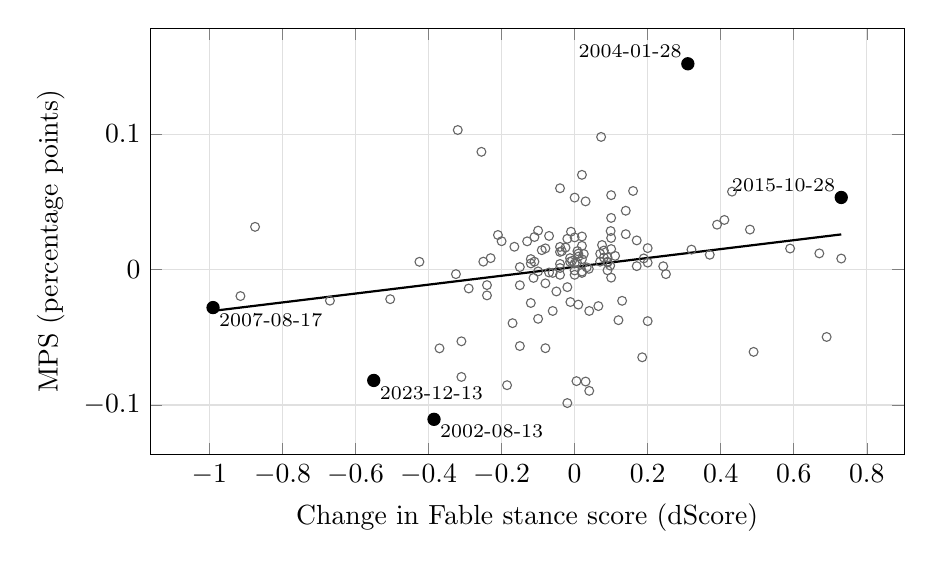
\begin{tikzpicture}
\begin{axis}[width=0.92\linewidth, height=7cm, xlabel={Change in Fable stance score (dScore)},
  ylabel={MPS (percentage points)}, ymajorgrids, xmajorgrids, major grid style={black!12}, clip=false]
\addplot[only marks, mark=o, mark size=1.6pt, black!60] coordinates {(-0.5050,-0.0219) (0.0000,0.0237) (0.0000,0.0531) (-0.0900,0.0143) (-0.8750,0.0315) (0.4100,0.0366) (0.4900,-0.0608) (-0.1000,-0.0364) (-0.2000,0.0209) (-0.0400,-0.0039) (0.4800,0.0295) (-0.0400,0.0600) (-0.1200,0.0077) (-0.1850,-0.0854) (0.0400,-0.0306) (0.0000,0.0044) (0.0300,-0.0827) (0.1400,0.0434) (-0.1500,-0.0565) (0.7300,0.0081) (-0.1200,-0.0247) (-0.0100,0.0279) (0.0200,-0.0015) (0.0100,-0.0259) (0.0000,-0.0007) (0.0400,-0.0896) (0.0300,0.0503) (0.0200,0.0244) (-0.0800,-0.0102) (0.6900,-0.0498) (-0.2400,-0.0191) (-0.3200,0.1030) (0.0900,-0.0006) (-0.0800,-0.0581) (0.1400,0.0261) (0.1000,0.0549) (0.1000,-0.0060) (-0.0200,-0.0986) (-0.0200,-0.0130) (0.1000,0.0151) (0.1000,0.0381) (-0.0600,-0.0306) (-0.0400,0.0011) (-0.0800,0.0156) (-0.0500,-0.0162) (-0.0700,-0.0022) (-0.1100,0.0058) (0.0900,0.0052) (0.0200,-0.0025) (0.2000,0.0158) (-0.0600,-0.0025) (0.0800,0.0140) (-0.2400,-0.0115) (0.0200,0.0699) (0.1000,0.0233) (0.0200,0.0175) (-0.1500,-0.0116) (0.1700,0.0215) (-0.0400,0.0130) (-0.1000,0.0287) (-0.0200,0.0227) (-0.1100,0.0240) (0.0900,0.0089) (-0.0400,0.0041) (0.0900,0.0058) (0.0100,0.0117) (0.0200,0.0076) (0.3700,0.0109) (-0.2500,0.0058) (0.0000,-0.0039) (0.0800,0.0088) (0.6700,0.0119) (-0.2300,0.0084) (-0.2100,0.0255) (0.0700,0.0116) (-0.0400,0.0167) (0.1700,0.0025) (-0.0700,0.0248) (0.3900,0.0331) (-0.3100,-0.0530) (-0.1000,-0.0014) (0.1850,-0.0648) (-0.4250,0.0057) (0.2000,-0.0381) (0.2500,-0.0034) (-0.3700,-0.0582) (-0.6700,-0.0230) (0.0050,-0.0824) (0.0750,0.0181) (-0.1700,-0.0396) (0.5900,0.0155) (0.1300,-0.0231) (0.0250,0.0115) (-0.2900,-0.0140) (-0.1300,0.0208) (-0.3250,-0.0034) (0.1600,0.0580) (-0.0350,0.0136) (-0.0250,0.0162) (-0.1500,0.0018) (-0.1200,0.0045) (-0.1650,0.0168) (-0.9150,-0.0196) (0.0650,-0.0270) (0.1200,-0.0374) (-0.3100,-0.0793) (0.2000,0.0051) (0.0077,0.0136) (-0.0116,-0.0240) (0.0974,0.0029) (0.0062,0.0051) (0.0331,0.0016) (-0.0126,0.0084) (-0.0124,0.0057) (0.0107,0.0096) (-0.0070,0.0064) (0.0388,0.0005) (0.0697,0.0058) (0.0986,0.0284) (0.1108,0.0101) (0.1892,0.0082) (0.3199,0.0147) (0.4309,0.0575) (0.2426,0.0024) (0.0725,0.0979) (-0.2552,0.0869) (-0.1126,-0.0062)};
\addplot[only marks, mark=*, mark size=2.2pt, black] coordinates {(-0.3850,-0.1106) (0.3100,0.1519) (-0.9900,-0.0281) (0.7300,0.0532) (-0.5500,-0.0819)};
\addplot[domain=-0.990:0.730, samples=2, thick, black] {0.00196 + 0.03283*x};
\node[font=\scriptsize, anchor=north west, inner sep=2pt] at (axis cs:-0.3850,-0.1106) {2002-08-13};
\node[font=\scriptsize, anchor=south east, inner sep=2pt] at (axis cs:0.3100,0.1519) {2004-01-28};
\node[font=\scriptsize, anchor=north west, inner sep=2pt] at (axis cs:-0.9900,-0.0281) {2007-08-17};
\node[font=\scriptsize, anchor=south east, inner sep=2pt] at (axis cs:0.7300,0.0532) {2015-10-28};
\node[font=\scriptsize, anchor=north west, inner sep=2pt] at (axis cs:-0.5500,-0.0819) {2023-12-13};
\end{axis}
\end{tikzpicture}

\caption{MPS against Fable's dScore at \R{prim.n} hold meetings, 2000--2023, with the fitted line of the
primary regression. Filled points: the five meetings whose removal lowers the $t$-statistic most.}\label{fig:scatter}
\end{figure}

\paragraph{Subperiods and other checks.} Table~\ref{tab:extra} reports exploratory checks that an
independent review asked for. The relation is concentrated in the last third of the sample: the
$t$-statistic is \R{extra.sub0007.t} for 2000--2007 ($n=\R{extra.sub0007.n}$), \R{extra.sub0815.t} for
2008--2015 ($n=\R{extra.sub0815.n}$) and \R{extra.sub1623.t} for 2016--2023 ($n=\R{extra.sub1623.n}$). The
score level, rather than its change, is not significantly related to MPS ($t=\R{extra.level.t}$).
Controlling for the previous statement's MPS or for the previous dScore leaves the $t$-statistic at
\R{extra.lagmps.t} and \R{extra.lagds.t}, so the result does not come from persistence in either series.
The concentration in 2016--2023 coincides with the period in which the Chair held a press conference
after every meeting from 2019; the 30-minute window of MPS largely precedes the press conference, but the
daily yield changes include it, and I do not control for it.

\begin{table}[t]
\centering
\caption{Exploratory checks}\label{tab:extra}
\footnotesize
% generated by paper/make_tables.py - do not edit
\begin{tabular}{@{}l rrrr l@{}}
\toprule
Check (outcome MPS, hold meetings) & $n$ & $\hat\beta$ & NW $t$ & $p$ & Sample \\
\midrule
Subperiod 2000--2007 & 32 & 0.036 & 1.32 & 0.196 & 2000-06--2007-08 \\
Subperiod 2008--2015 & 58 & 0.012 & 0.42 & 0.673 & 2008-06--2015-10 \\
Subperiod 2016--2023 & 42 & 0.049 & 3.40 & 0.002 & 2016-01--2023-12 \\
\addlinespace[3pt]
Score level instead of its change & 132 & 0.010 & 1.38 & 0.170 & 2000-06--2023-12 \\
\addlinespace[3pt]
Primary + previous statement's MPS (dScore coef.) & 132 & 0.033 & 2.39 & 0.019 & 2000-06--2023-12 \\
Primary + lagged dScore (dScore coef.) & 132 & 0.033 & 2.29 & 0.024 & 2000-06--2023-12 \\
\addlinespace[3pt]
Joint: paraphrased dScore & 132 & 0.015 & 0.98 & 0.331 & 2000-06--2023-12 \\
\quad and clean $-$ paraphrased & 132 & 0.045 & 3.59 & $<$0.001 & 2000-06--2023-12 \\
\addlinespace[3pt]
Joint: blinded dScore & 132 & 0.021 & 1.83 & 0.070 & 2000-06--2023-12 \\
\quad and clean $-$ blinded & 132 & 0.060 & 2.25 & 0.026 & 2000-06--2023-12 \\
\addlinespace[3pt]
Outcome MPS $-$ MPS\_ORTH (predictable part) & 125 & 0.022 & 4.99 & $<$0.001 & 2000-06--2023-12 \\
MPS on the same meetings & 125 & 0.033 & 2.39 & 0.018 & 2000-06--2023-12 \\
\addlinespace[3pt]
Primary, $x$ and $y$ winsorised at 2.5/97.5\% & 132 & 0.034 & 2.54 & 0.012 & 2000-06--2023-12 \\
\bottomrule
\end{tabular}

\tabnote{\emph{Notes:} Outcome MPS (or its predictable part, MPS $-$ MPS\_ORTH), hold meetings, policy
corpus, Newey--West $t$. All rows except the joint rows use Fable's consensus dScore; ``coef.'' rows
report the dScore coefficient in a regression with the stated control. Joint rows: MPS regressed in one equation on Fable's single-prompt dScore from the paraphrased
(or blinded) text and on the difference between the clean and the paraphrased (blinded) dScore. These
checks were added after the primary specification was frozen and count towards the regression total.}
\end{table}

\paragraph{Information beyond the surprise.} Does dScore tell us anything about yields that the surprise
does not? It does not. Adding dScore to
a regression of daily yield changes on MPS raises the $R^2$ by between \R{beyond.fable.gainmin} and
\R{beyond.fable.gainmax} percentage points, with no $|t|$ above \R{beyond.fable.tmax} (Appendix
Table~\ref{tab:beyond}).

\subsection{Fable against Gemini}

Gemini's dScore correlates with Fable's at \R{corr.fable.gemini}, yet on its own it has no relation to any
market outcome. Table~\ref{tab:gemini} puts both in one regression, with each dScore standardised. Fable's
coefficient has $t$-statistics between \R{j.tFmin} and \R{j.tFmax}, and Gemini's turns negative, between
\R{j.tGmin} and \R{j.tGmax}. With two correlated regressors this joint regression is close to a
regression on the difference between them: the market-related information sits in the part of Fable's
score change that Gemini does not share. The negative Gemini coefficient does not mean that Gemini's score
is informative with the wrong sign. The difference between the two models' standardised slopes, estimated
from separate regressions, has a block-bootstrap $z$ between \R{j.zmin} and \R{j.zmax}
\citep[moving blocks of four meetings, 2{,}000 draws;][]{kunsch1989}, and every 95\% interval excludes
zero. Without the five meetings most influential for the primary result (Table~\ref{tab:influence}), the
joint $t$-statistics are between \R{jdrop.tFmin} and \R{jdrop.tFmax} for Fable and between \R{jdrop.tGmin}
and \R{jdrop.tGmax} for Gemini, and the gap $z$ is between \R{jdrop.zmin} and \R{jdrop.zmax}. These
comparisons were added after the primary specification was frozen and lie outside its family, so they
are exploratory.

\begin{table}[t]
\centering
\caption{Fable against Gemini, hold meetings}\label{tab:gemini}
\small
% generated by paper/make_tables.py - do not edit
\begin{tabular}{@{}l r rr rr rrr@{}}
\toprule
 & & \multicolumn{2}{c}{Joint: Fable} & \multicolumn{2}{c}{Joint: Gemini} & \multicolumn{3}{c}{Gap in per-SD slopes} \\
\cmidrule(lr){3-4}\cmidrule(lr){5-6}\cmidrule(l){7-9}
Outcome & $n$ & $\hat\beta$ & NW $t$ & $\hat\beta$ & NW $t$ & Gap & $z$ & 95\% interval \\
\midrule
MPS & 132 & 0.020 & 3.41 & $-$0.014 & $-$2.66 & 0.008 & 2.23 & [0.002, 0.016] \\
$d_{2}$ & 120 & 3.11 & 2.76 & $-$2.94 & $-$3.32 & 1.60 & 2.59 & [0.30, 2.70] \\
$d_{10}$ & 120 & 2.94 & 3.09 & $-$2.20 & $-$3.32 & 1.36 & 2.56 & [0.38, 2.45] \\
$t_{2}$ & 132 & 2.42 & 3.21 & $-$1.84 & $-$2.79 & 1.00 & 2.38 & [0.24, 1.87] \\
$t_{10}$ & 132 & 1.90 & 3.33 & $-$1.43 & $-$3.33 & 0.78 & 2.46 & [0.27, 1.50] \\
\bottomrule
\end{tabular}

\tabnote{\emph{Notes:} Both dScores standardised on the common hold meetings. Joint: one regression of
the outcome on both, Newey--West $t$. Gap: Fable's minus Gemini's per-standard-deviation slope from
separate regressions; $z$ and the 95\% percentile interval from a moving-block bootstrap over meetings in
time order (block length 4, 2{,}000 draws). MPS in percentage points, yields in basis points, per
standard deviation of dScore.}
\end{table}

The difference between the two models is therefore suggestive, and more than a difference in
significance. It has two readings. Fable may read the statements better. Or it may know more about them,
including what followed. Section~\ref{sec:recognition} shows that Fable recognises the statements.
Gemini never names a date while scoring, but it was not given the dating probe, so whether it could
recognise them is untested. The human labels below help to tell the readings apart, but only a little.

\subsection{Agreement with human labels}

\begin{table}[t]
\centering
\caption{Correlation of score levels with published human sentence labels}\label{tab:tdw}
\small
% generated by paper/make_tables.py - do not edit
\begin{tabular}{@{}l rr rr@{}}
\toprule
 & \multicolumn{2}{c}{All statements} & \multicolumn{2}{c}{Hold meetings} \\
\cmidrule(lr){2-3}\cmidrule(l){4-5}
Score & $n$ & $r$ & $n$ & $r$ \\
\midrule
Claude Fable 5.1 (five prompts) & 100 & 0.459 & 76 & 0.366 \\
Gemini 2.5 Flash (five prompts) & 100 & 0.511 & 76 & 0.516 \\
Dictionary word count & 100 & 0.309 & 76 & 0.199 \\
GPT-4 (P1) & 97 & 0.514 & 73 & 0.455 \\
\bottomrule
\end{tabular}

\tabnote{\emph{Notes:} Statements with at least two sentences that appear word for word among the
hand-labelled sentences of \citet{shah2023} (hawkish $+1$, neutral 0, dovish $-1$); $r$ is the correlation
of the model's score level with the mean label, \R{tdw.first}--\R{tdw.last}. GPT-4 lacks scores for three
statements.}
\end{table}

If Fable's edge over Gemini came from better reading, Fable should also agree better with human readers.
Table~\ref{tab:tdw} compares each score's level with the mean of the human labels of \citet{shah2023} on
the \R{tdw.n} statements with at least two labelled sentences. All three LLMs agree moderately with the
labels, and Fable does not agree best: its correlation is \R{tdw.fable.r}, against \R{tdw.gemini.r} for
Gemini and \R{tdw.gpt4.r} for GPT-4, and \R{tdw.fable.rhold} against \R{tdw.gemini.rhold} and
\R{tdw.gpt4.rhold} on hold meetings. The dictionary reaches \R{tdw.dict.r}.

This benchmark is limited. The labels were made for sentences, not statements; only a few sentences per
statement are labelled, many of them boilerplate; and the test is on levels, while the market test is on
changes. The labelled sentences differ between neighbouring statements, so a change test with these labels
mostly measures which sentences happen to be labelled (all models' correlations with the change in the mean
label are between \R{tdw.fable.rchg} and \R{tdw.gemini.rchg}). Within these limits, the human benchmark does
not single out Fable as the better reader. Its market edge is not matched by an edge in agreement with
humans, which fits ``knows more'' at least as well as ``reads better''.

\subsection{Blinded and paraphrased text}\label{sec:versions-validity}

It is tempting to read the fall in the MPS $t$-statistic from \R{hold.clean.MPS.t} on the clean text to
\R{hold.blind.MPS.t} on blinded and \R{hold.para.MPS.t} on paraphrased text as evidence that recalled
information was removed. The evidence is mixed. The falls are not clearly significant: of the
\R{g.n} bootstrap gaps between the clean slope and the blinded or paraphrased one (three outcomes, two
text versions), with $z$-statistics between \R{g.zmin} and \R{g.zmax}, only \R{g.over196} has $|z|$
above 1.96 (the $d_2$ gap for blinding), and every 95\% percentile interval includes zero
(Appendix Table~\ref{tab:gaps}). Recognition on request hardly changes: Fable still dates
\R{probe.blind.exactpct} of blinded and \R{probe.para.exactpct} of paraphrased statements. But
recognition while scoring does fall: Fable names the statement's month and year in
\R{spont.cleanfable.all.pct} of its P1 replies on the clean text, \R{spont.blindfable.all.pct} on blinded
and \R{spont.parafable.all.pct} on paraphrased text. And paraphrasing removes legitimate information:
markets react to exact wording such as ``considerable period'' or ``patient'', which a paraphrase must
change.

The last point can be made concrete. Splitting the clean dScore into the paraphrased dScore and the
difference between the two, and entering both in one regression for MPS, gives a $t$-statistic of
\R{extra.decpara.t} for the paraphrased part and \R{extra.decparares.t} for the difference
(Table~\ref{tab:extra}); for blinding the figures are \R{extra.decblind.t} and \R{extra.decblindres.t}.
The market-related part of the score is concentrated in what paraphrasing and blinding change. For the
paraphrase, that fits both readings: exact wording carries information, and identity cues may trigger
recall. Blinding is more telling, because it leaves the wording of the policy paragraphs intact and
removes mainly dates, names, vote rosters and named events. That the part of the score blinding removes is
related to MPS ($t=\R{extra.decblindres.t}$) points towards identity cues, or towards the context they
carry, rather than towards wording. This is the strongest indication of recall in the paper. It is weak
evidence: the blinded and clean dScores correlate at \R{corr.clean.blind}, the check is
exploratory, and the gap between the clean and blinded slopes is not significant on its own.

\subsection{Summary}

Fable's dScore has a positive and small relation to the policy surprise at hold meetings. It changes
little with how the score is built or how the corpus is defined, it is not driven by outliers, and its
sensitivity to influential meetings is what a real effect of this size would show. But it does not survive
a multiple-testing correction, it was found after a specification search, and it is concentrated in
2016--2023. The daily yield link depends on the corpus definition. Fable outperforms Gemini on market
data but not on human labels. None of this separates reading from remembering, and the one check that
leans either way (the part of the score that blinding removes) leans towards remembering.
